\documentclass{llncs}
\pdfoutput=1
\pagestyle{plain}

\usepackage{booktabs}

\usepackage{algorithm, algpseudocode}
\usepackage{relsize}

\renewcommand{\tabcolsep}{2pt}


\renewcommand{\algorithmiccomment}[1]{/*#1*/}
\usepackage{epsfig, endnotes, url}
\usepackage{color, cite, graphicx}
\usepackage{mathtools, amsmath, amsfonts}
\usepackage{diagbox, booktabs, colortbl}
\usepackage{multirow, subcaption}
\usepackage{breakurl, listings, framed}
\usepackage[hidelinks]{hyperref}
\usepackage{xspace}
\usepackage{slashbox}
\usepackage{enumitem, array}
\DeclareMathAlphabet{\mathcal}{OMS}{cmsy}{m}{n}

\captionsetup[subfigure]{justification=raggedright}

\newcolumntype{?}{!{\vrule width 1pt}}

\captionsetup{compatibility=false}
\def\UrlBreaks{\do\/\do-}
{\renewcommand{\arraystretch}{1.2}
\makeatletter
\newcommand{\@chapapp}{\relax}%
\makeatother

\usepackage[title]{appendix}

\newcommand{\tabitem}{~~\llap{\textbullet}~~}

\newcommand{\ignore}[1]{}
\newcommand\ghada[1]{\nbc{GA}{#1}{teal}}
\newcommand\david[1]{\textbf{\textcolor{blue}{[david] #1}}}
\newcommand\derek[1]{\textbf{\textcolor{green}{[derek] #1}}}
\newcommand{\fake}[1]{{\color{magenta} [fake: #1]}}
\usepackage{array}
\newcolumntype{P}[1]{>{\centering\arraybackslash}p{#1}}

\begin{document}

\title{\Large \bf Confirm Service Activity in the NuCypher Network}
\author{Ghada Almashaqbeh}

\institute{NuCypher \\
\email{ghada@nucypher.com}}
\date{} % delete this line to display the current date



\maketitle

\begin{abstract}
In this document we introduce several aspects related to the confirm activity problem in 
the NuCypher network. These include the different definitions of this problem, the 
underlying threat model, the current adopted solution, and its relation 
to both service fees and inflation rewards. In particular, we consider two flavors of the confirm activity issue, namely, confirm availability 
and confirm service activity. The former confirms that Ursula is available all the time 
and replies to all requests coming from Bob, while the latter provides a proof that an 
Ursula has served a specific number of distinct re-encryption 
requests within a given a period. We present potential solutions 
for each of these flavors and discuss at 
what stage of the network operation they are likely to be used.
\end{abstract}

\section{Introduction}
\label{intro}
The NuCypher network~\cite{egorov2017nucypher} is a decentralized key management 
system, encryption, and access control service. It uses proxy re-encryption, namely, the 
Umbral scheme~\cite{umbral2018}, to delegate access to encrypted 
documents through a public network. This network is composed of a set of semi-trusted 
re-encryption servers, or Ursulas, that implement access control policies created by data 
owners, or Alices. Alice supplies each Ursula with re-encryption keys allowing Ursula to transform 
ciphertexts encrypted under Alice's public key into ciphertexts encrypted under the delegatee's, or Bob's,
public key. This enables the latter to decrypt the ciphertext without revealing anything about the
decryption keys or the raw data to the intermediate servers.


Joining the NuCypher network is governed by consensus rules defining the service setup
and the monetary incentives paid to provide the service. In order to join the 
system, Ursula needs to stake an amount of NU tokens for a specific period
which will be released when the pre-specified staking period is over. Alice chooses an
Ursula to hold an access control policy with a probability proportional to the stake this Ursula 
pledged in the system. Therefore, the stake value influences the amount of service load an Ursula
may receive. This stake is also used to punish Ursula financially, by revoking part 
of it, if she cheats and this cheating is detected. 


Alice joins the network by creating a policy to be implemented by a 
set of Ursulas. This policy specifies the re-encryption key fragments each Ursula will
need to answer requests coming from Bob(s), as well as the duration of the policy, which 
is basically the timeframe during which Bob is authorized to access Alice's data.  Furthermore,
Alice will lock an amount of Ether into the policy to be used to pay Ursulas for the re-encryption 
service. As noted, Alice is not exposed to the NU token. All that she needs is an Ethereum
wallet, awareness of the NuCypher network architecture to select Ursulas, and knowledge of the
NuCypher rules of preparing access control policies.


Bob, on the other hand, does not deal with currency in the system. It interacts with the storage 
network to retrieve the encrypted data, and with Ursulas in the NuCypher network to request the
re-encryption service.


\subsection{Monetary Incentives in the NuCypher Network}
Ursulas are rewarded for the re-encryption service by using two sources; 
the first is the service fees collected from the policy  
owner Alice, while the second is inflation rewards, i.e., newly minted
NU tokens, coming from the NuCypher network. The latter will be provided during the 
early stage of the network operation to encourage 
adoption. It is expected that these rewards will disappear as the token cap is 
reached, similar to other cryptocurrencies in the space.


Currently, the inflation rewards for each round or period are computed for each Ursula based on the size of her stake given that she confirms to be online during this round. Confirming the status of being online is done by calling a 
simple function in one of the NuCypher contracts, which is like a signal that the calling Ursula is online.

As for fees, Ursula collects part of the Ether locked by Alice during the policy's duration in proportion to the number of periods up to that point in which Ursula has confirmed her online status. 


\subsection{Problems with Current Reward Computation Approach}
The current approach of computing Ursula's inflation rewards and service fees suffers from two
main problems:
\begin{itemize}
\setlength{\itemsep}{0pt}
\item The rewards computation (both fees and inflation) is agnostic to the number of 
requests Ursula serves. Thus, an active Ursula who may serve a huge number of 
re-encryption requests, and one who does not receive any requests (or a
malicious/lazy Ursula that does not answer Bob's requests), will 
both collect the same amount of rewards if they hold identical policies.

\item Confirming being online is flawed in the sense that this function does 
not require any input or proofs from Ursula on providing the service. Ursula 
can stay offline and not respond to Bobs' requests, but come online merely to call the confirm activity
function. This allows Ursula to collect both inflation rewards 
and fees without doing any work. Even worse, Ursula will be able to get her stake back once she unlocks its her stake (i.e., when policies being managed by Ursula expire). 
\end{itemize}



\subsection{Problem Statement}
The confirm activity problem is defined differently based on the stage of the 
NuCypher network. In early network operation, when inflation rewards are 
still distributed, we are concerned with the availability of Ursulas and being willing to 
serve all requests coming from Bob. In other words, regardless of the number of 
requests served, the rewards value will be computed based on the period during which Ursula 
is online and well-behaving. While in later stages, when inflation rewards disappear 
and only fees exist, confirm activity will be tied to providing the re-encryption 
service in the sense that the payment will be computed based on the amount of 
service provided. Thus, Ursula needs to confirm its activity by proving that she served 
a given number of distinct re-encryption requests during a given period. To make the distinction 
clear, we refer to the first as confirm availability, and for the second as confirm 
service activity.


In this document, we introduce several solutions for both forms of confirming activity. 
These solutions differ in the trust, efficiency, interactivity, and resource 
requirements, in addition to their security guarantees. We divide the document into 
two parts, the first is about confirm availability, while the second is about confirm 
service activity. We begin with outlining the adopted threat model for each problem 
definition, as well as the network model. Then, we present the proposed solutions, discuss the aforementioned
trade-offs and requirements of each of them, with the goal of selecting one of these 
solutions to be adopted for each stage of the NuCypher network operation.


\subsection{Threat and Network Models}
\label{threat-network-model}
This section describes a modification for the network model of NuCypher 
required by the proposed solutions, in 
addition to the threat model adopted in this work.


\subsubsection{Network Model.}
In order for the proposed solutions to work, we need to ensure freshness, 
integrity, and authenticity of the requests (as well as service complaints as we will see later) issued by Bob. This can be achieved 
by requiring Bob to sign each re-encryption request it issues and to include a timestamp, or 
sequence number, in each request to ensure freshness. The keypair used for the 
signature should be separate from the keypair Bob uses for proxy encryption in the 
system. 


Until now we assume that Alice pays for the service by using the Ether she locks 
in the policy contract. Other arrangement may emerge in the system like having 
Bob pay for each requests he issues. Such an arrangement and its implication on the 
confirm activity issue will be studied once it becomes part of the NuCypher 
network protocol.


\subsubsection{Threat Model.}
In our threat model, we make the following set of assumptions:
\begin{itemize}
\item {\bf Self-interested parties:} We do not place trust in any party and we assume that all participants are 
self-interested. This means that a party may decide to 
follow the protocol or deviate from it, either on its own or by colluding 
with other attackers, and such decision is solely based on what maximizes the financial profits
of this party.

\item {\bf Attackers' collusion:} If it is profitable, an Ursula may, for example, spin out  
its own Alice and/or Bob or collude with Alice. We do not consider collusion 
between Bob and Ursula as a practical threat. This means that cases of Bob pretending  
that he got service from Ursula (while no service is delivered) is not an issue. We do not 
suspect this will be of any importance and there is no motivation to do it given that 
the work Ursula does for re-encryption is minimal.

The above non-collusion assumption does not affect the solutions proposed to handle 
the confirm service activity discussed in Section~\ref{confirm-service-activity}. This 
means that these solutions provide higher 
security guarantees and address the issue of potential collusion between Bob and Ursula. 
It could be the case that relaxing the requirement of 
addressing this collusion case allows deploying more efficient solutions. 
In order to make an educated decision of the plausibility of this threat, we need 
more data about the system operation and the behavior of the participants 
once the inflation rewards disappears in the system. Therefore, we leave this 
issue until later when fees become the only source of rewards for Ursulas.

\item {\bf Honest Ursulas:} We also assume that when sampling a subset of Ursulas in the network, 
at least one of them is honest. This assumption can be achieved by 
having a global assumption regarding the lower bound of the number of 
honest Ursulas with respect to the total number of Ursulas in the system. 
(Or it can be achieved by deploying a special entity like an external verifier, 
that changes on a periodic basis, or one by the NuCypher company, that is
trusted to faithfully participate as a member of each samples set. This 
verifier does not provide any other services 
in the system.)
\end{itemize}


Other than the above, we have usual assumptions like dealing with 
computationally bounded adversaries 
that cannot break secure cryptographic primitives with non-negligible probability. 
(We may need to work in the random oracle model, but this depends on the 
security requirements of the proposed solutions.)




\section{Threat and Network Models}
\label{threat-network-model}
This section describes a modification for the network model of NuCypher 
required by the proposed confirm service activity solutions, in 
addition to the threat model we adopt in this document.


\subsection{Network Model}
In order for the proposed solutions to work, we need to ensure freshness, 
integrity, and authenticity of the requests issued by Bob. This can be achieved 
by requiring Bob to sign each request it issues and to include a timestamp, or 
sequence number, in each request to ensure freshness.

\david{NuCrypher currently supports this by allowing Bob to include a blockhash,
although it's not being used for the moment.}

The following approach can be used here; given that Umbral already requires Bob to 
have a key pair, this pair can be used for signing and verifying the signed requests. 
This also means that Ursula should be aware the secret key can be used for 
signing the requests and the public 
key should be known to Ursula to verify the signatures. 

\david{Reusing the same keypair for encryption and signing may introduce some key management problems. Is it possible to find a solution that supports separate keypairs?}

\subsection{Threat Model}
We do not place trust in any party and we assume that all participants are 
self-interested. This means that a party may 
follow the protocol or deviate from it, either on its own or by colluding 
with other attackers, is solely based on what maximizes the financial profits 
of this party. As such, Ursula may collude with Bob or Alice (by spinning 
its own Alice and/or Bob for example) to achieve her financial goals. 


We also assume that when sampling a subset of Ursulas in the network, 
at least one of them is honest. This assumption can be achieved by 
having a global assumption regarding the lower bound of the number of 
honest Ursulas with respect to the total number of Ursulas in the system. 
(Or it can be achieved by deploying a special entity like an external verifier, 
that changes on periodic basis, or one by the NuCypher company, that is 
trusted to faithfully participate in the confirm 
service activity protocol. This verifier does not provide any other services 
in the system.)


Other than the above, we have usual assumptions like dealing with 
computationally bounded adversaries 
that cannot break secure cryptographic primitives with non-negligible probability. 
(We may need to work in the random oracle model, but this depends on the 
security requirements of proposed solutions.)

\section{Preliminaries}
\label{prelim}
This section provides an overview of two concepts that we use in the 
proposed solutions. These include the framework of proof carrying data (PCD) 
and the collective signing (CoSi) protocol.


\subsection{Proof Carrying Data (PCD)}
The paradigm of PCD~\cite{chiesa2010proof} allows proving to the correctness of a distributed 
computation involving untrusted parties. It produces a single proof for the output 
that attests not only the correctness of the final result, but also 
the correctness of the entire history of intermediate computations that produced 
this result. Correctness here is defined as a polynomially computable predicate that 
abstracts the properties, or invariants, that must be satisfied.


\begin{figure}[h!]
\centerline{
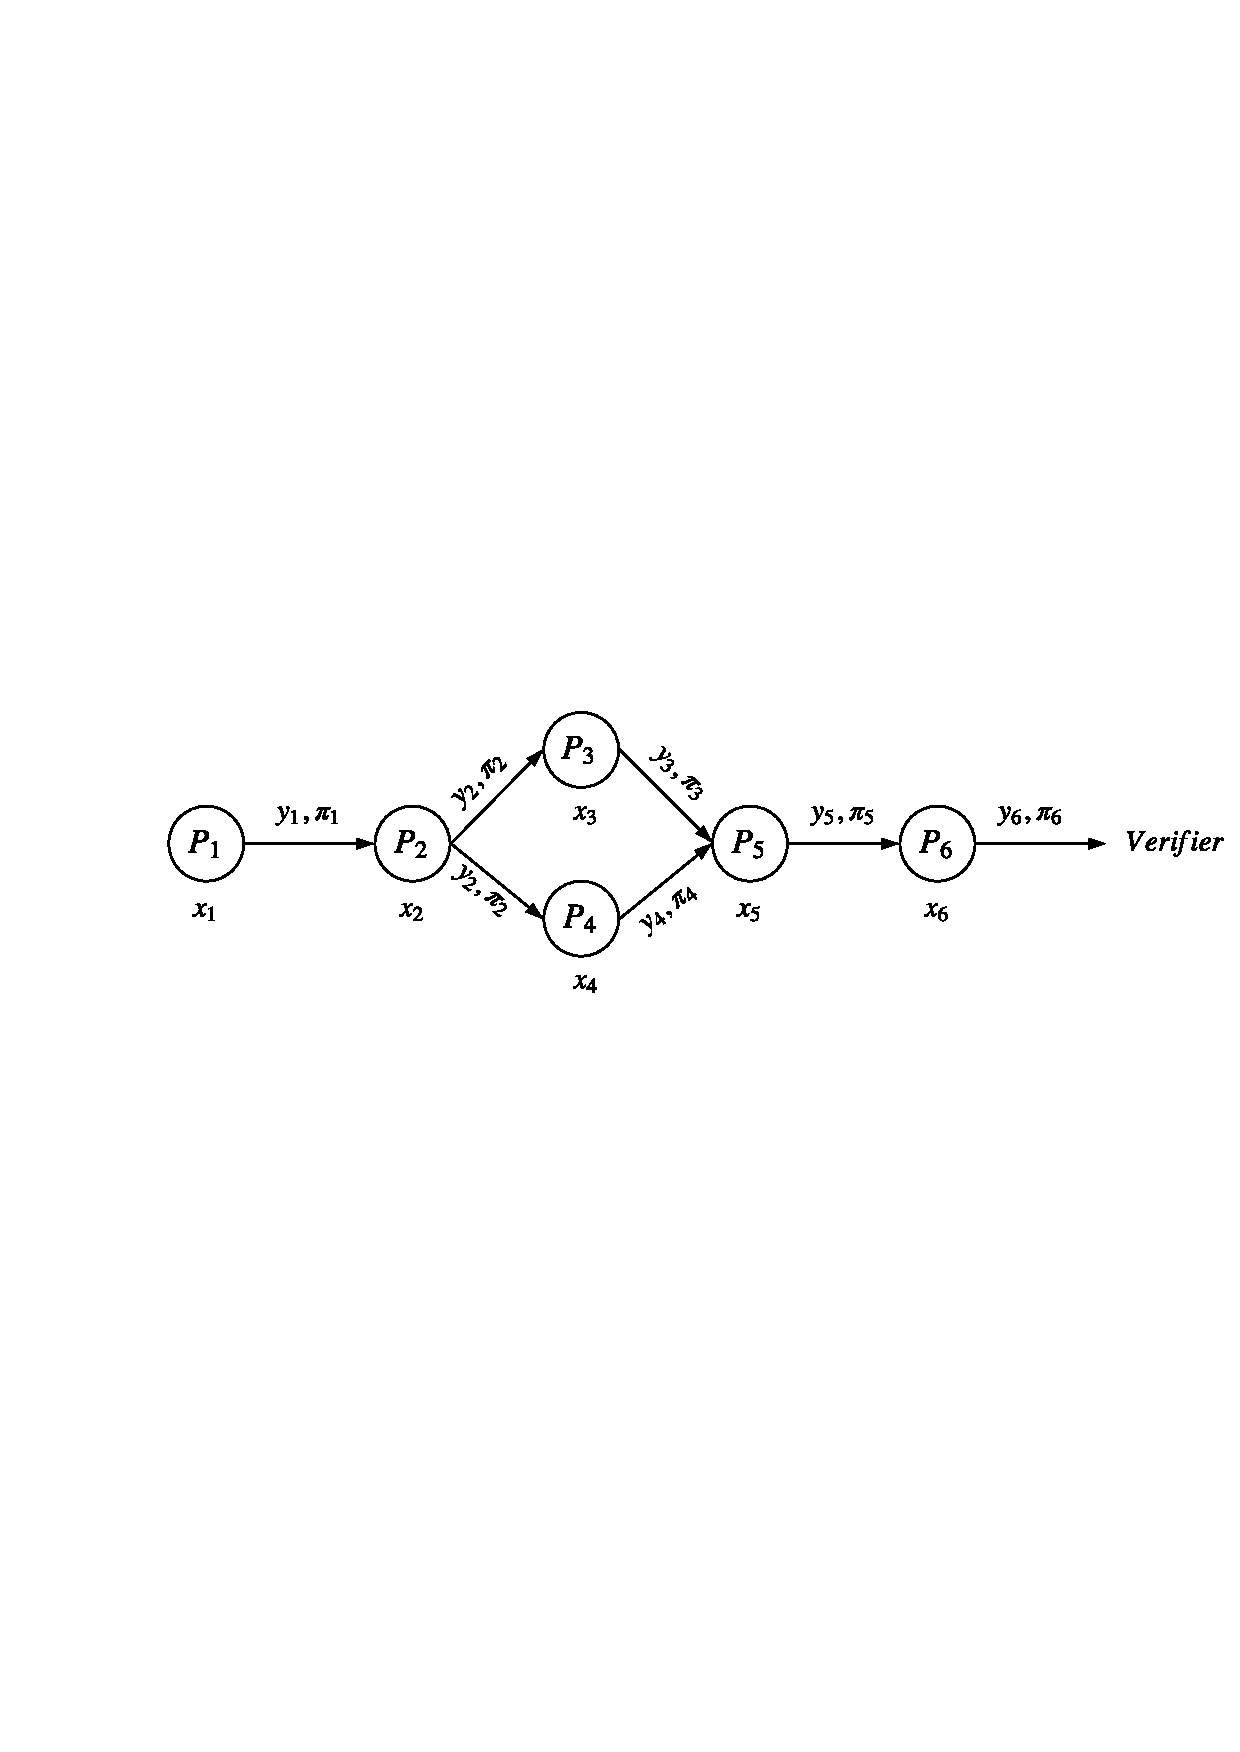
\includegraphics[height= 1.3in, width = 1.0\columnwidth]{figures/pcd-diagram.pdf}}
\caption{An example of a PCD application. A distributed computation involving parties $P_i$, for 
$i \in \{1, \dots, 6\}$, each 
of which has a local input $x_i$ and produces an output $y_i$ with a proof $\pi_i$. }
\label{pcd-diagram}
\end{figure}


To clarify how PDC works, consider a distributed computation task that involves 
the set of parties shown in Figure~\ref{pcd-diagram}. Party $P_1$ starts the computation with its 
own input, produces an intermediate output with a proof saying that it performed 
the computation as defined by the protocol. It then sends both the output and the proof 
to the next party, which is $P_2$ in this case. Here, $P_2$ will 
have its own input $x_2$, as well as everything it received from $P_1$ (including the proof) 
as input to the computation it will perform. Similarly, $P_2$ will produce another 
intermediate output and a proof. This proof not only attests to the correctness of the 
computation done by $P_2$, but also the history that lead to the result $y_2$. In other 
words, it implicitly includes 
the proof from $P_1$. The same process continues until the full computation is finished. 
Anyone can verify the correctness or compliance of the whole distributed protocol by 
only verifying the last proof $\pi_6$ produced by the exit party, which is $P_6$ in the figure.


As shown, PCDs enable untrusted parties to work with each other in a fully distributed 
fashion, without overwhelming the system with the storage and verification of individual 
proofs for each step of the performed protocol. Also, they attest to correctness or compliance  
to the prescribed protocol without re-executing any of the intermediate computations. Thus, 
they provide a promising paradigm for confirming service activity in a compact way.


\subsection{Collective Signing (CoSi)}
\label{cosi}
CoSi~\cite{syta2016keeping} is a protocol that enables a set of distributed parties to cosign a 
statement together in a way that produces a single signature. As such, both the 
verification time and the space requirements are just like having a single signer. The 
difference is that this signature attests that all parties agree with the signed 
statement instead of only one.


CoSi builds upon Schnorr 
multisignatures~\cite{schnorr1991efficient, bellare2006multi, micali2001accountable}, but combines 
them with communication trees to speed up the signing process in 
case of a large number of cosigners. In what follows, we only present the protocol
with a plain communication architecture as it suffices for the confirm service activity 
solution introduced in this document.


Schnorr signatures work in a group $\mathbb{G}$ of a prime order $q$ and 
generator $g$, such that the discrete log is believed to be hard in this group. 
Take $n$ parties that want to sign a statement together. 
Each of these parties has a secret $sk_i \in \mathbb{Z}_q$ and a public key 
$pk_i \in \mathbb{G}$ such that $pk_i = g^{sk_i}$. To sign a message $m$, 
one of these parties, let's say $P_1$, coordinates the signing process as follows: 
\begin{enumerate}
\setlength{\itemsep}{0pt}
\item $P_1$ prepares a message $m$ and sends it to the rest of the signers.

\item Each party $P_i$, possibly after verifying 
$m$, selects a secret $\tau_i \in \mathbb{Z}_q$ and compute $V_i = g^{\tau_i}$, 
then it sends $V_i$ back to $P_1$.

\item $P_1$ aggregates all random values received from 
the signers, and its own, by computing $V = \Pi_{i =1}^n V_i$.

\item $P_1$ then computes 
$c = H(V||m)$, where $H$ is an appropriate hash function. $P_1$ then 
sends $c$ to the rest of the parties.

\item Each party computes a response $r_i = \tau_i - sk_i\cdot c$ and 
sends it to $P_1$.

\item Lastly, $P_1$ computes $r = \sum_{i=1}^n r_i$, and outputs the 
collective signature over $m$ as $(c, r)$.
\end{enumerate}


Verifying the signature proceeds as in classical Schnorr signatures~\cite{schnorr1991efficient} with 
one difference. An aggregated public key $pk$ is used in the verification process, 
which is computed as $pk = \Pi_{i=1}^{n} pk_i$.


The work in~\cite{syta2016keeping} tackles several issues related to 
the availability of the 
signing parties, and optimizing the communication between them. 
We believe that such techniques can be used in the NuCypher network if we adopt the 
CoSi-based solution for the confirm service activity issue.


\section{Potential Solutions}
\label{solutions}
This section outlines several potential solutions for how to let Ursula prove 
that she served a given number of distinct requests in a publicly verifiable way. 
One of these solutions, the PCD-based one, is still a work in progress. The goal 
is to share the high-level idea of each of these solutions and to chose the best one,
after we define the meaning of best, to be adopted by the NuCypher network.


\subsection{PCD-based Scheme}
The main idea here is to adapt the PCD framework so that Ursula
can combine the correctness proofs she computes for Bobs' requests in a single proof 
attesting to the following fact: ``Ursula has served $\omega$ distinct re-encryption 
requests correctly." 


Thus, in this setup, there is only one computation party, or prover, namely, Ursula. 
For each round, where a round could be the time needed to mine a block on the 
blockchain, Ursula starts with input $x_1$, which is a signed and fresh request
from Bob. It answers this request with $cFrag_{x_1}$ and produces a correctness 
proof $\pi_1$ as defined in the Umbral scheme, in addition to another correctness 
proof $\hat{\pi}_1$ that will be used in the PCD composition. Then, when the next request $x_2$ arrives, 
which is the input for the next step in the computation, Ursula answers 
this request as before and produces $cFrag_{x_2}$ and a correctness proof $\pi_2$, then 
it uses $(x_2, cFrag_{x_2}, \pi_2)$ and the previous proof $\hat{\pi}_1$ to produce $\hat{\pi}_2$. 
$\hat{\pi}_2$ does not only 
attest to the correctness of $cFrag_{x_2}$, but also attests to the fact that Ursula has served 
two valid distinct requests until now. The same process is repeated until the end of the 
round to produce a single proof $\hat{\pi}_{\omega}$ along with the number of 
served requests $\omega$. Figure~\ref{pcd-based-sol} depicts 
this process pictorially.


\begin{figure}[h!]
\centerline{
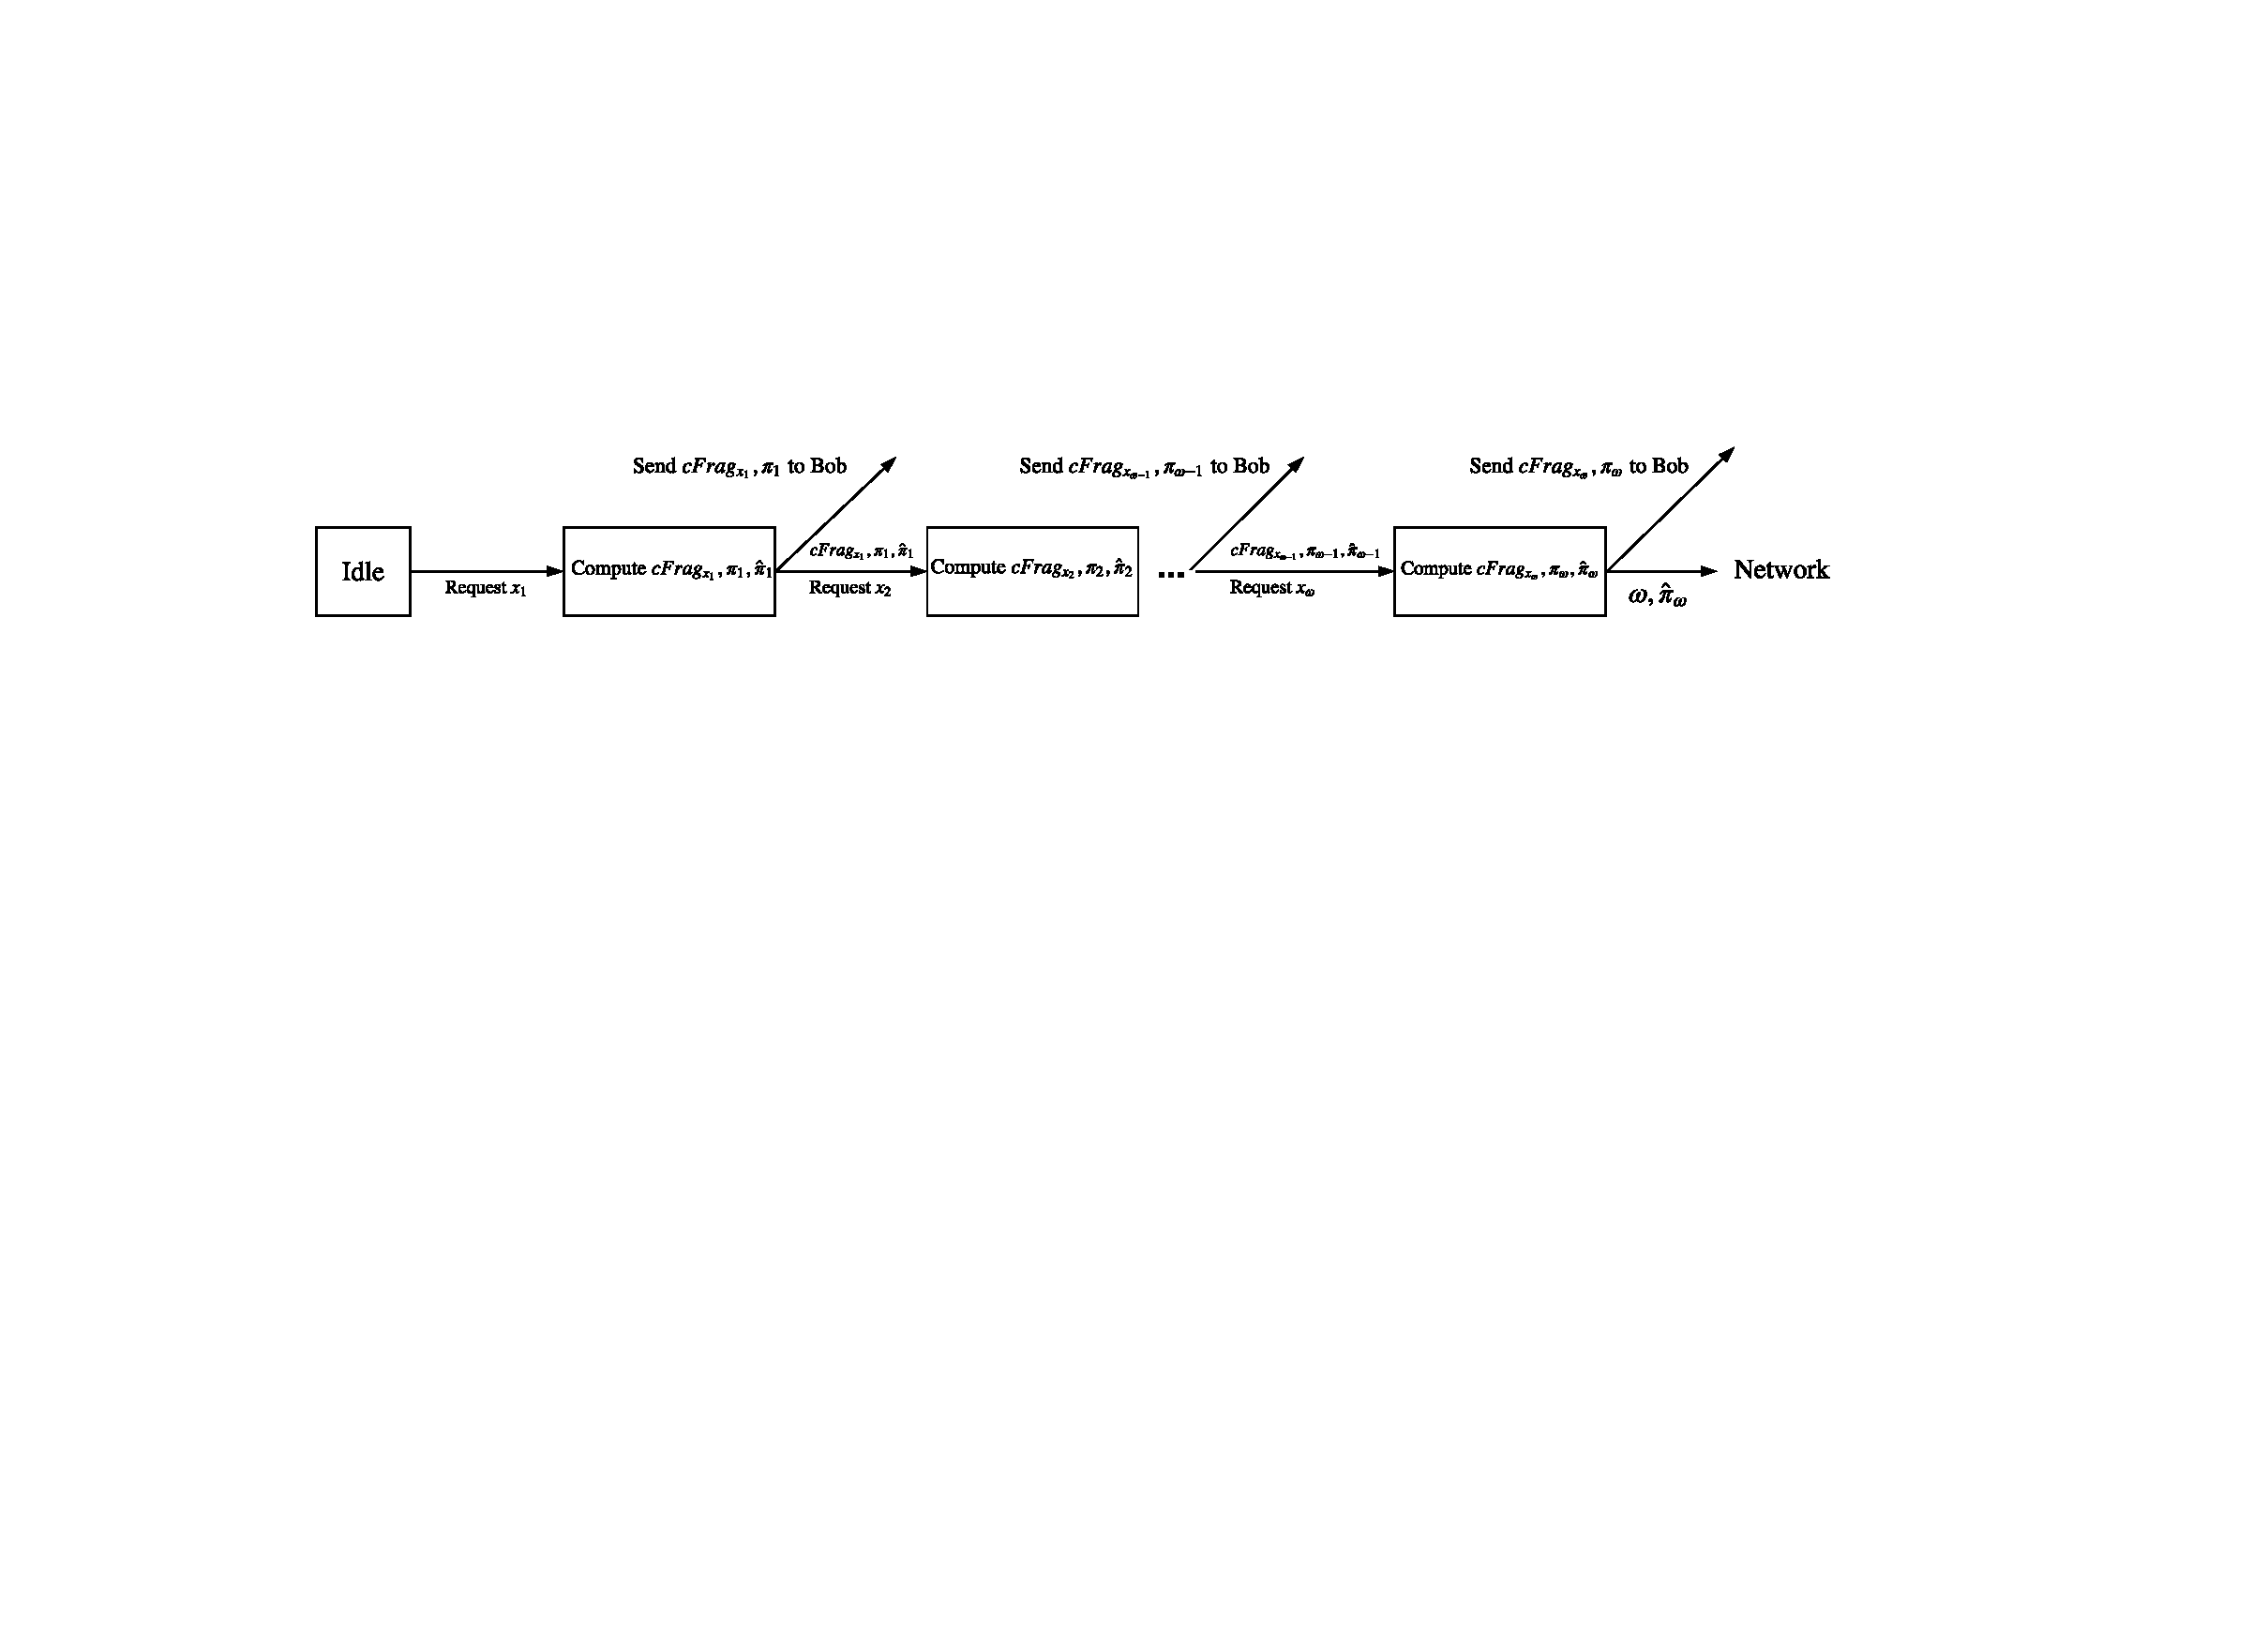
\includegraphics[height= 0.7in, width = 1.0\columnwidth]{figures/pcd-based-sol.pdf}}
\caption{PCD-based solution diagram. Ursula starts a round in the idle state. When 
the first request arrives, Ursula responds to the request and starts composing the 
proofs as new requests arrive. At the end of the round, Ursula announces the number of 
served requests and a single proof attesting to its claim to the network. }
\label{pcd-based-sol}
\end{figure}


The final proof will be processed by the contract that governs Alice's policy. A valid proof 
allows Ursula to claim fees out of Alice's Ether escrow as a payment for $\omega$ re-encryption  
requests. 


The above is a high level description of the idea. However, more time is need to 
understand PCD and SNARKs in order to come up with a concrete construction 
(if possible). Please see Section~\ref{future-work} for more information.

\david{I think it is possible to aggregate current Umbral proofs. I started to explore this option in the past but there was no use for it at that moment.}

\subsection{CoSi-based Scheme}
This solution utilizes the idea of collective signing by electing a committee 
that will sign a report submitted by a specific Ursula after verifying that 
the report supports the claim that ``Ursula has served $\omega$ distinct 
re-encryption requests correctly." 


At a high level, the scheme works as follows. For each round, a working Ursula keeps 
a full record of all the requests that she served during the round. These 
include the signed requests received from Bob(s), and the produced $cFrag$ 
and the correctness proof $\pi$ (as in the Umbral scheme) for 
each request. At the end of the round, a committee of $t$ Ursulas is 
elected, where $t$ is a small integer, e.g., $t = 5$. The working Ursula 
initiates the CoSi protocol to sign the message $m$ stated above while 
replacing $\omega$ with the actual number of served 
requests in the round. This Ursula sends $m$ along with the full report to 
each member in the committee. Each member Ursula (i.e., member in the 
elected committee) verifies $m$ by checking the report as follows:
\begin{enumerate}
\setlength{\itemsep}{0pt}
\item Check that each request is distinct and valid by verifying Bob's 
signature over the request. (Here the policy will contain Bob's public 
key to allow the committee use the right verification key.)

\derek{Signature only validates request, but for distinct requests, presumably blockhash/sequence number needs to also be checked?}

\item Verify the correctness of each $cFrag$ as in the Umbral 
scheme.

\item Check that the value of $\omega$ inside $m$ agrees with the 
record.
\end{enumerate}


If everything is fine, each member of the committee and the working 
Ursula finalize the CoSi signing protocol as described in Section~\ref{cosi}. 
At the end, the working Ursula publishes the collective signature, which can be 
verified using the accumulated public keys of the cosigning Ursulas.


\subsubsection{On the committee election.} This can be done
by using some deterministic computation over a block hash and mapping
the output to Ursulas' public keys. So the selection is not determined by the
working Ursula to prevent any potential collusion. The selection may also take into account the presence and size of each Ursula's stake, to avoid an attacker spinning up enormous numbers of Ursulas in order to increase the chance of them controlling the entire committee.


The above scheme works under the assumption that at least one Ursula
in the elected committee is honest, which pertains to an assumption on the
least number of honest Ursulas in the network. If the latter assumption is under threat, one mitigating approach is to increase $t$ (the committee size).


Another approach is to have a changing set of external verifiers, like
trusted partners, that all working Ursulas must use for the CoSi signing
of their records.


A third approach is to keep the deterministic selection of the committee
but with an external member, e.g., either a trusted partner verifier
or a special verifier node deployed and maintained by the NuCypher company.
Thus, achieving the assumption of at least one member of the elected
committee is honest.


\subsubsection{On the publicity of the signed records.} Having a 
valid collective signature from a committee (that has at least one honest 
member) suffices for the correctness of the signed statement. However, 
it could be better to keep the records that produced the message $m$  
available for a while so that any party can verify them (the verifying
parties could maintain such a public record for a given period after which
the logs can be discarded). 


We can resort to this option just at the beginning to convince the 
participants of the trustworthiness of the committee or the validity of the
assumption that at least one Ursula in the elected committee is honest.


\subsubsection{On compensating the committee.} This solution may 
raise the question of why would the elected committee (especially if it 
is composed of other Ursulas in the system) participate in the CoSi 
process, which also involves verifying the full request record presented 
by the working Ursula. This can be pictured as a collaborative
work, the committee does the work so that others will do the same
when the committee members play the role of working Ursulas.


Another option is to pay the committee for their work, either as
part of the inflation rewards, or by having working Ursulas pay for 
it (however, this may complicate the system operation).


\subsection{Challenge/Open-based Scheme}
This solution utilizes the idea of commit/challenge/open protocols. 
In details, Ursula keeps track of the requests coming from Bob(s) 
during a time round and assign each of them a unique sequence 
number. That is, Ursula replies with $cFrag$ and the correctness proof 
along with a sequence number showing the order of the request within 
the batch of requests handled during a round. At the end of the round, 
Ursula constructs a Merkle tree of all requests, where 
the requests (and their replies) are the leaves of the tree ordered by the sequence
numbers. Ursula signs the root of the tree, denoted as $root$ to produce 
a signature $\sigma_{root}$, then it publishes $(\omega, root, \sigma_{root})$ 
to the network (recall that $\omega$ is the number of served requests). 


To prove correctness, Ursula will be challenged to open some leaves in the Merkle tree. 
This can be done by having the policy contract select at random (e.g. based
on the block hash or any other mechanism) the leaf IDs to be opened. If 
Ursula fails to open them correctly within a predefined timeframe, she loses the 
whole fee she was supposed to collect for serving $\omega$ requests.


An alternative approach to the challenge/open scheme described above is to 
have Ursula publish the full Merkle tree on some known public space but
not on the blockchain, and make the full record available online for a specific period
to allow anyone to verify the work. If no one files a complaint about the tree (we
still need to define correctness properties, like checking all Bob public keys are 
defined in the policy created by Alice, and that the response is valid by checking the 
proof produced by Umbral), Ursula collects the fees for the provided service. On the other
hand, a valid complaint or proof-of-cheating costs Ursula the full allocation of fees, or potentially involves slashing her stake.
\section{Discussion and Analysis}
\label{analysis}
Here we will discuss the security, financial, and performance implications of the 
proposed solutions in order to choose the best.


This will be delayed after discussing with the team to avoid biasing opinions 
about the proposed schemes.

\section{Future Work}
\label{future-work}
Most of the future work on the confirm service activity issue 
will be dedicated to construct a concrete PCD-based solution. This 
includes the following:
\begin{itemize}
\item Understand PCD and its applications in a greater depth. This 
also requires exploring NIZK in general and SNARKs in specific. 

\item Define an efficient output correctness predicate that characterizes 
the correctness of the statement that PCD will attest for. This could be 
hard for the confirm activity issue as the value of the output is dynamic 
based on the workload Ursula may receive.

\item Define a way to compose the proofs efficiently and produce 
a single proof at the end. This will be tied to the formulated predicate.

\item Argue about the correctness and security of the concrete scheme.
\end{itemize} 


The above will take time, but the good news that this will be also helpful 
to the work on PPSC. So it is more like developing part of the  
background needed for PPSC.



\bibliographystyle{unsrt}       % APS-like style for physics
\bibliography{confirmBib}
\end{document}